\documentclass{beamer}
%
% Choose how your presentation looks.
%
% For more themes, color themes and font themes, see:
% http://deic.uab.es/~iblanes/beamer_gallery/index_by_theme.html
%
\mode<presentation>
{
  \usetheme{default}      % or try Darmstadt, Madrid, Warsaw, ...
  \usecolortheme{default} % or try albatross, beaver, crane, ...
  \usefonttheme{default}  % or try serif, structurebold, ...
  \setbeamertemplate{navigation symbols}{}
  \setbeamertemplate{caption}[numbered]
} 


\usepackage[english]{babel}
\usepackage[utf8x]{inputenc}
\usepackage{listings}
\usepackage{graphicx}
\title[Template Tutorial Presentation]{Template Tutorial Presentation}
\author{Emily}


\begin{document}

\begin{frame}
  \titlepage
\end{frame}

% Uncomment these lines for an automatically generated outline.
%\begin{frame}{Outline}
%  \tableofcontents
%\end{frame}

\section{Introduction}

\begin{frame}{Introduction}

\begin{itemize}
  \item This template tutorial is meant to be guide for setting up tutorial packages 
  \item By the end of walking through this package you should feel comfortable packing your own tutorial  
\end{itemize}


\end{frame}

\section{Some \LaTeX{} Examples}

\subsection{How to use the template tutorial}

\begin{frame}{ReadMe}

\begin{itemize}
  \pause \item Utilize the README as a way of orienting your user, how do you want them to go through the tutorial? What needs to be installed?
  \pause \item For the template tutorial the user should first read the README, install the requirements, and then read through this presentation. Finally, the user will go through the notebooks.
\end{itemize}

\end{frame}

\begin{frame}{Graph}

% Commands to include a figure:
%need to go to Project-->files --> upload a new file can't upload from desktop or docs
\begin{figure}
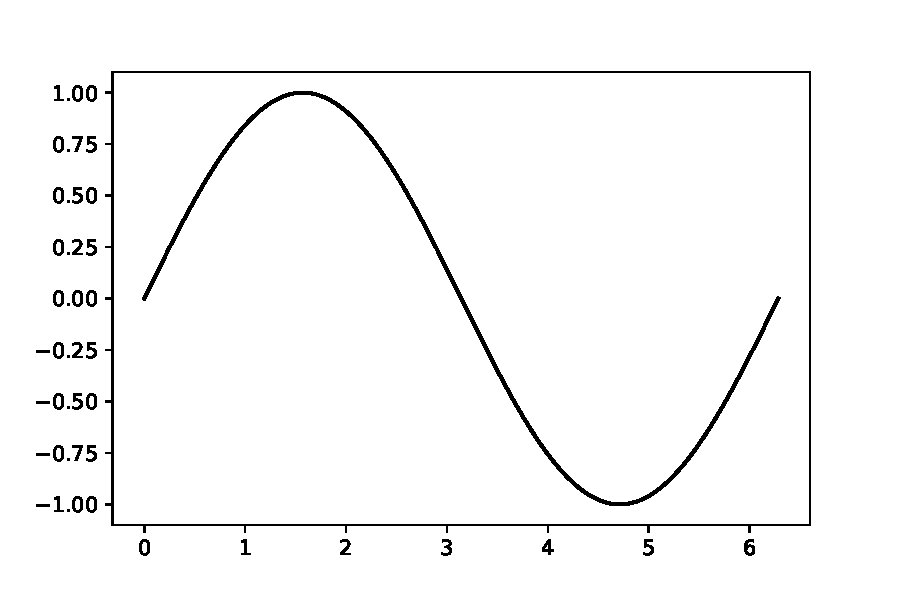
\includegraphics[width=\textwidth]{figs/sin} 
\caption{\label{fig:your-figure} A simple sine wave.}
\end{figure}
\end{frame}

\begin{frame}

\begin{figure}
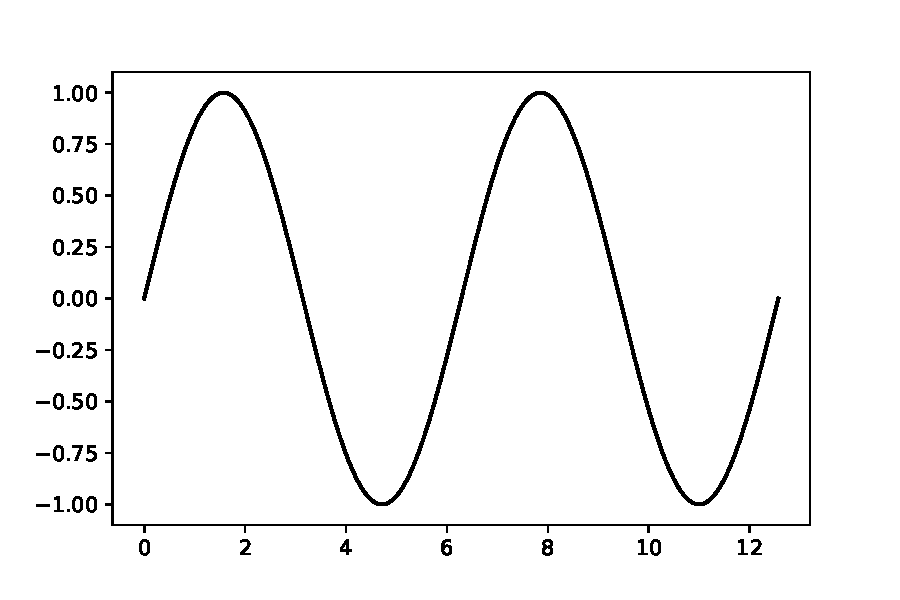
\includegraphics[width=\textwidth]{figs/2sin} 
\caption{\label{fig:your-figure} A sine wave with double the frequency.}
\end{figure}

\end{frame}{}

\subsection{Code}

\begin{frame}[fragile]{Code}

Here is an example of code from the "data" module. When making your own slide show you might want to highlight a snippet of code that would be most useful to the audience 

\begin{verbatim}
>>> import numpy as np
>>> import matplotlib.pyplot as plt
>>> x = np.linspace(0, 3*np.pi, 500)
\end{verbatim}

\end{frame}

\subsection{Summary}

\begin{frame}{Summary}

\begin{itemize}[<+->]
\item This tutorial should be a jumping off point for other tutorials. 
\item By cloning this repo you will have all the tools needed to create your own tutorial.
\item Good luck and thank you for teaching others!
\end{itemize}

\end{frame}

\end{document}

%\How to make a table
%\begin{table}
%\centering
%\begin{tabular}{l|r}
%Item & Quantity \\\hline
%Widgets & 42 \\
%Gadgets & 13
%\end{tabular}
%\caption{\label{tab:widgets}An example table.}
%\end{table}


